\documentclass[a4paper]{article}

\usepackage[english]{babel}
\usepackage[utf8]{inputenc}
\usepackage{amsmath}
\usepackage{graphicx}
\usepackage[colorinlistoftodos]{todonotes}
\usepackage[T1]{fontenc}	%ADDED for << og >>
\usepackage{enumitem}		%ADDED for smaller spacing

\newcommand{\tab}[1]{\hspace{.2\textwidth}\rlap{#1}}

\title{Assinment41}

\author{pebj, smot}

\date{\today}

\begin{document}
\maketitle

\section{OOSE}

\subsection{Specify relevant pre- and postconditions}

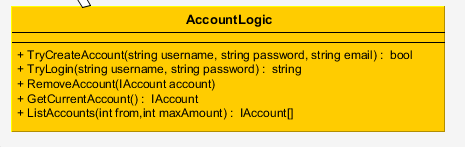
\includegraphics[scale = 1]{AccountLogic.png}

\noindent
/* To remove an account you have to be logged in as the account or\\
* be a moderater.*/\\
\textbf{context} AccountLogic::RemoveAccount(account) \textbf{pre:}
\begin{itemize}[noitemsep,nolistsep]
\item[] account.equals(Season.CurrentAccount()) or
\subitem Season.CurrentAccount()->IsModerater()\\
\end{itemize}

\noindent
/*The accounts refferences will become null\\
* The account will not be accessable in the database*/\\
\textbf{context} AccountLogic::RemoveAccount(account) \textbf{post:}
\begin{itemize}[noitemsep,nolistsep]
\item[] account.equals(null) and
\subitem OnlineContext.GetAccount(username) is ObjectNotFoundException\\
\end{itemize}

\noindent
/*The username may not exist in the databace\\
* you have to be online*/\\
\textbf{context} AccountLogic::TryCreateAccount(username, password, email) \textbf{pre:}
\begin{itemize}[noitemsep,nolistsep]
\item[] no Season.GetAccount(username) and
\subitem OnlineContext->isOnline()\\
\end{itemize}

\noindent
/*An account in the database will be created\\
* It will be possible to login with the new account afterwards*/\\   
\textbf{context} AccountLogic::TryCreateAccount(username, password, email)\textbf{post:}
\begin{itemize}[noitemsep,nolistsep]
\item[] Season.GetAccount(username).username.equals(username)
\subitem AccountLogic->TryLogin(username,password)\\
\end{itemize}


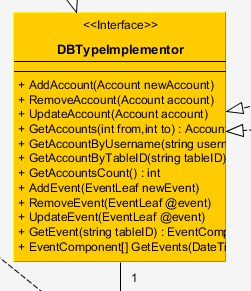
\includegraphics[scale = 1]{IMPLEMENTOR.png}

\noindent
/*The events TableID may not be ''''\\
* The given events TableID is valid*/\\
\textbf{context} DBTypeImplementor::UpdateEvent(event) \textbf{pre:}
\begin{itemize}[noitemsep,nolistsep]
\item[] not event.TableID.equals("") and
\subitem GetEvent(event.itemIndex).equals(a event)\\
\end{itemize}

\noindent
/*An updated event' content is equals the event from GetEvent(self.tableID);\\
* There will be a corresponding command in season*/\\   
\textbf{context} DBTypeImplementor::UpdateEvent(event) \textbf{post:}
\begin{itemize}[noitemsep,nolistsep]
\item[] GetEvent(event.tableID).equals(event)
\subitem Season.changeCommands->contains(UpdateEvent)\\
\end{itemize}


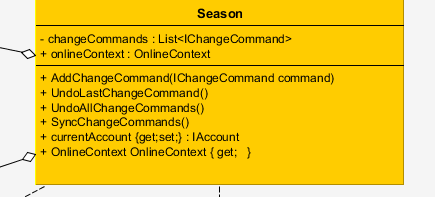
\includegraphics[scale = 1]{Season.png}

\noindent
/*The login account is a moderater*/\\
\textbf{context} Season::GetAccounts(from,to) \textbf{pre:}
\begin{itemize}[noitemsep,nolistsep]
\item[] CurrentAccount()->IsModerater() and
\subitem from > 0 and 
\subsubitem to < GetAccountsCount()\\
\end{itemize}

/*You will get an array containing all accounts from "from" to "to"*/\\
\noindent   
\textbf{context} Season::GetAccounts(from,to) \textbf{post:}
\begin{itemize}[noitemsep,nolistsep]
\item[] GetAccounts().length = to - from\\
\end{itemize}


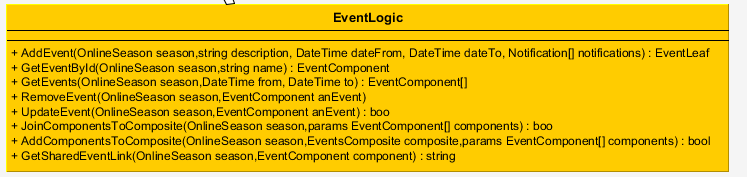
\includegraphics[scale = 1]{EventLogic.png}

\noindent
/*components contains at lest 2 EventComponent\\
* An account is loggetin*/\\
\textbf{context} EventLogic::JoinComponentsToComposite(OnlineSeason, components) \textbf{pre:}
\begin{itemize}[noitemsep,nolistsep]
\item[] components.length >= 2  and
\subitem not OnlineSeason.CurrentAccount().equals(null)\\
\end{itemize}

\noindent 
/*you will get an EventsComposite contaning all EventComponents\\
* in components\\
* There will be a corosponding command in OnlineSeason*/\\   
\textbf{context} EventLogic::JoinComponentsToComposite(OnlineSeason, components) \textbf{post:}
\begin{itemize}[noitemsep,nolistsep]
\item[] JoinComponentsToComposite(OnlineSeason, components).eventComponents->contains(components[0])
\subitem OnlineSeason.changeCommands->contains(UpdateEvent)\\
\end{itemize}


\subsection{Specify invariants}


\noindent
/*There can't be two referrencing to the same EventComponent's*/\\
*in an EventsComposite*/\\
\textbf{context} EventsComposite \textbf{inv:}
\begin{itemize}[noitemsep,nolistsep]
\item[] eventComponents.contains(x => x).where(x == event).Count() = 1\\
\end{itemize}

\noindent
/* An account have to be logged in to use EventLogic*/\\
\textbf{context} EventLogic \textbf{inv:}
\begin{itemize}[noitemsep,nolistsep]
\item[] OnlineSeason.CurrentAccount() != null\\
\end{itemize}

\noindent
/* If there is internet connection, OnlineContext uses Online. Otherwise,\\
* OnlineContext uses Offline*/\\
\textbf{context} OnlineContext \textbf{inv:}
\begin{itemize}[noitemsep,nolistsep]
\item[] if isOnline() then
\subitem	\_syncStrategy is Online
\item[] else
\subitem	\_syncStrategy is Offline\\
\end{itemize}

\subsection{Object Model}
The Object model below is a splitted up version of the original so as to have space for it in this document. The complete one image version of the Object Model can be seen in the same folder as this document.


\begin{table}
\centering
	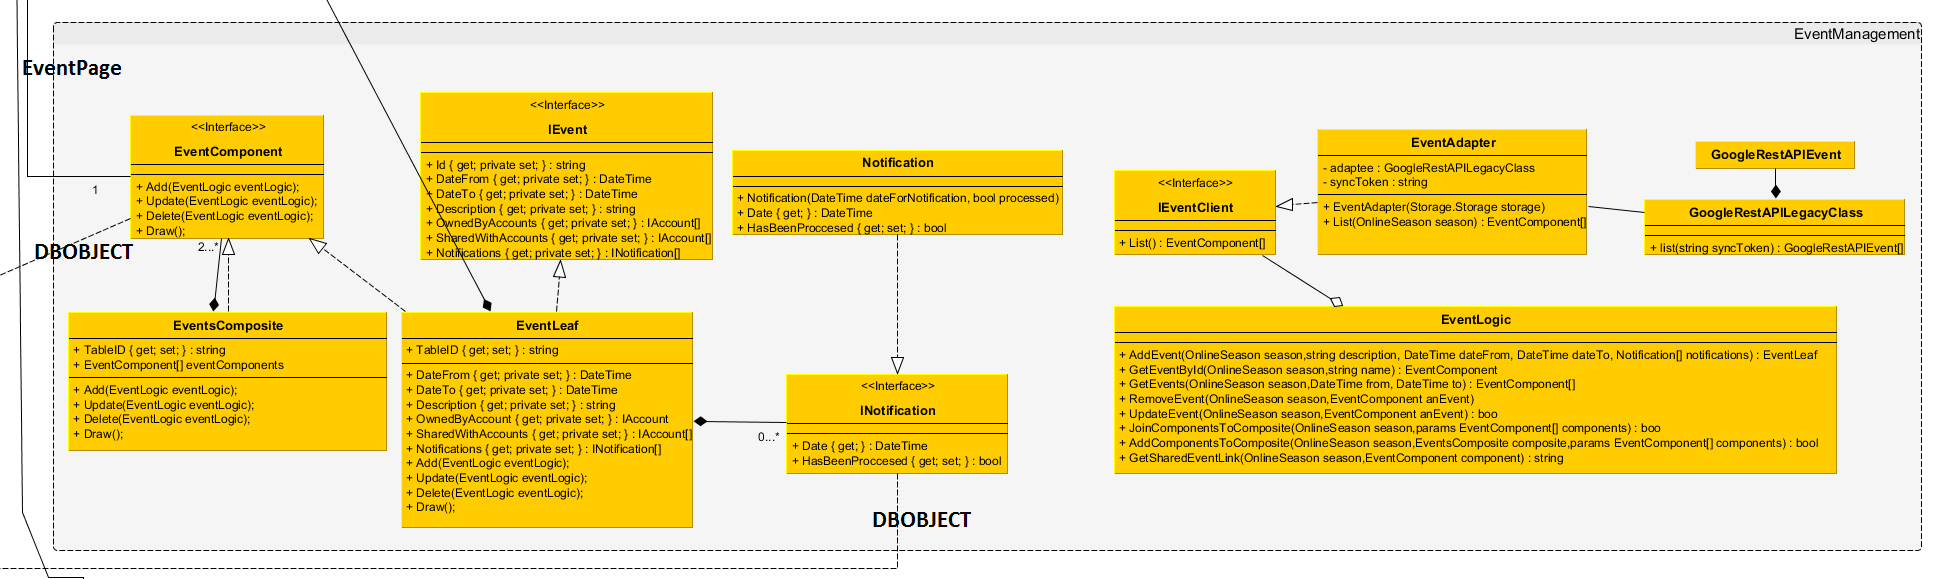
\includegraphics[width=1.3\textwidth]{EventManagement.png}\\
\caption{\textbf{EventManagement}}
\end{table}

\begin{table}
\centering
	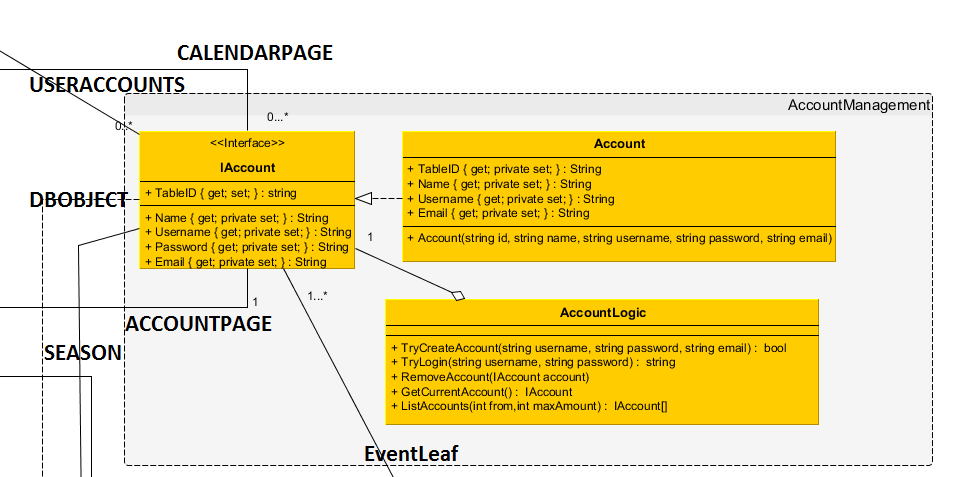
\includegraphics[width=1.3\textwidth]{AccountManagement.png}\\
\caption{\textbf{AccountManagement}}
\end{table}

\begin{table}
\centering
	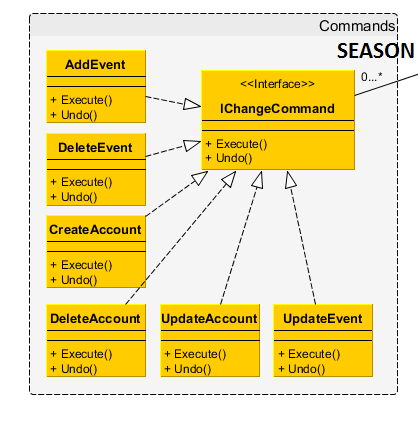
\includegraphics[width=0.8\textwidth]{Commands.png}\\
\caption{\textbf{Commands}}
\end{table}

\begin{table}
\centering
	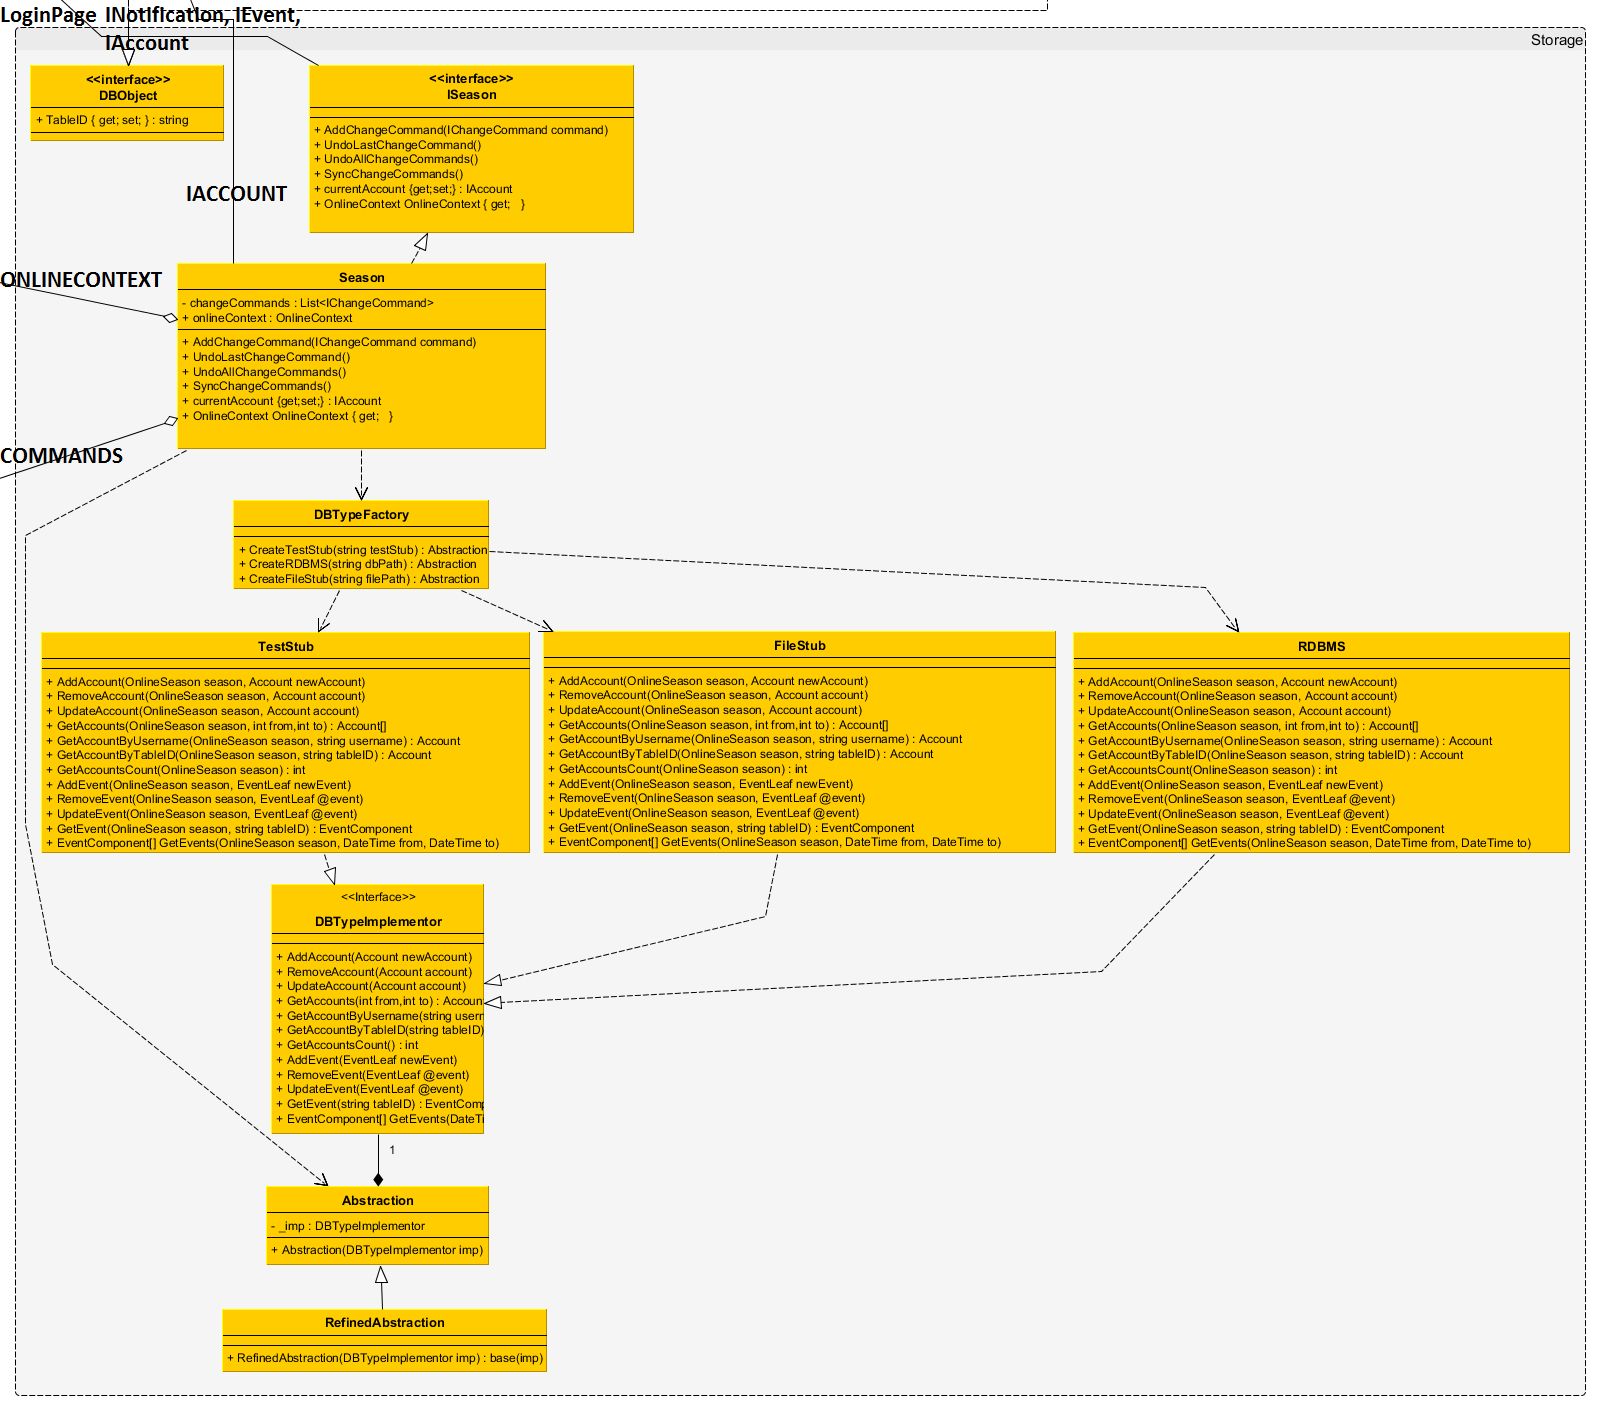
\includegraphics[width=1.3\textwidth]{Storage.png}\\
\caption{\textbf{Storage}}
\end{table}

\begin{table}
\centering
	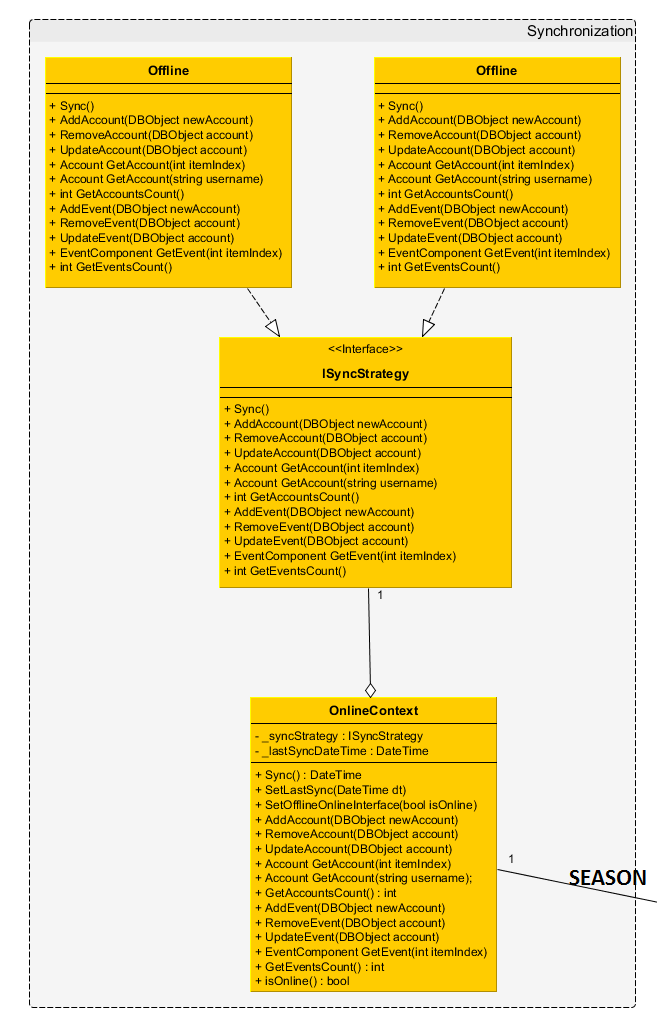
\includegraphics[width=1.3\textwidth]{Synchronization.png}\\
\caption{\textbf{Synchronization}}
\end{table}

\begin{table}
\centering
	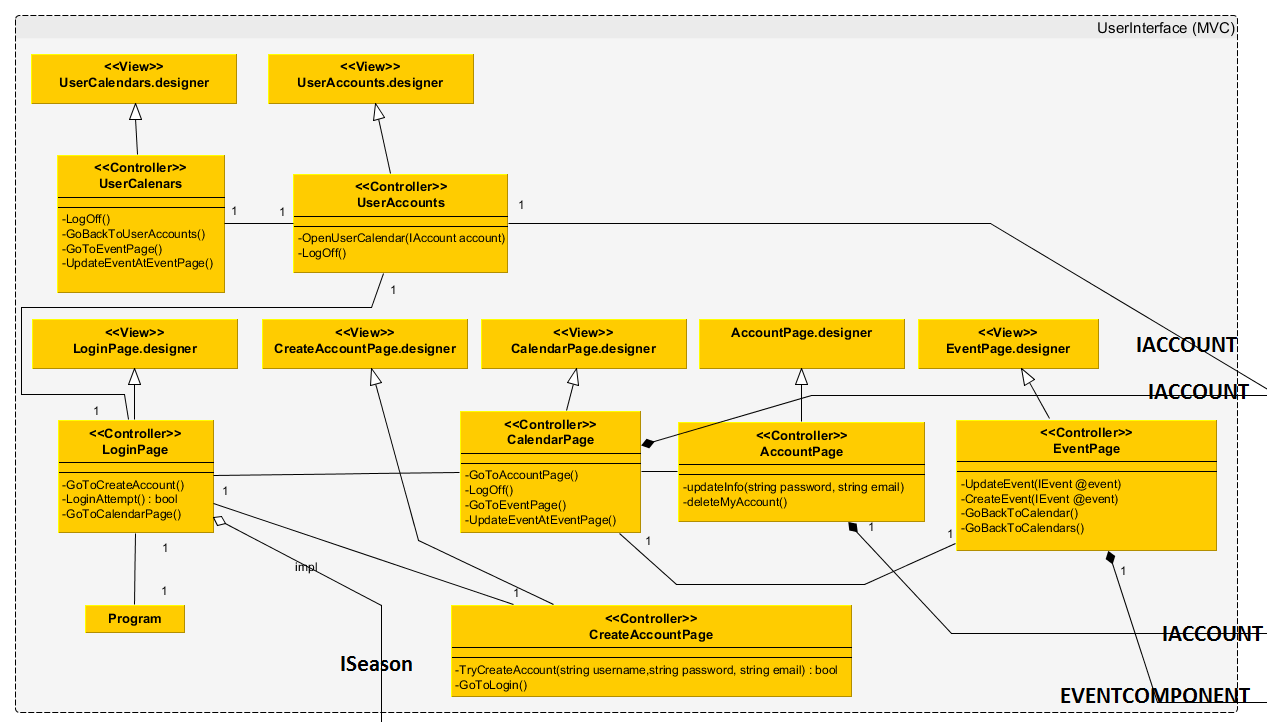
\includegraphics[width=1.3\textwidth]{UserInterfaceMVC.png}\\
\caption{\textbf{UserInterface\_MVC}}
\end{table}

\begin{table}
\centering
	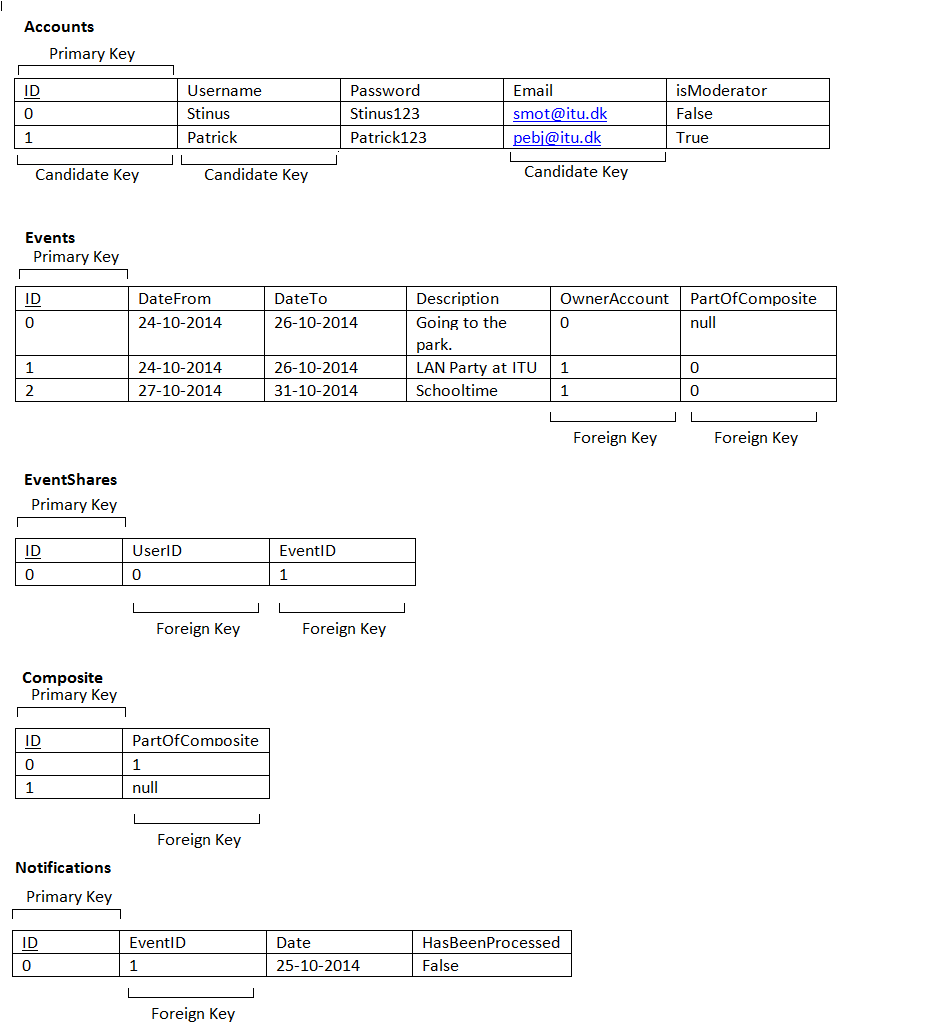
\includegraphics[width=1.3\textwidth]{tables.png}\\
\caption{\textbf{OO-to-RDBMS mapping}}
\end{table}


\end{document}